\begin{figure}[H]
	\centering
	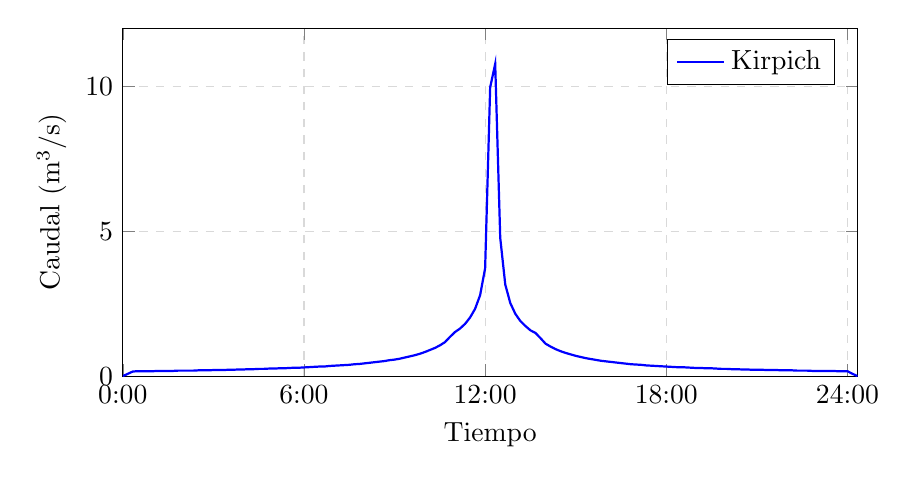
\begin{tikzpicture}
		\begin{axis}[
			width=0.9\textwidth,
			height=6cm,
			xlabel={Tiempo},
			ylabel={Caudal (m$^3$/s)},
			xmin=0,
			xmax=1460,
			ymin=0,
			ymax=12,
			grid=major,
			grid style={dashed, gray!30},
			legend pos=north east,
			xtick={0, 360, 720, 1080, 1440},
			xticklabels={0:00, 6:00, 12:00, 18:00, 24:00},
			]
		% Kirpich
		\addplot [
		blue,
		thick,
		solid,
		] coordinates {
				(0, 0.00) (10, 0.08) (20, 0.16) (30, 0.17) (40, 0.17)
				(50, 0.17) (60, 0.17) (70, 0.18) (80, 0.18) (90, 0.18)
				(100, 0.18) (110, 0.19) (120, 0.19) (130, 0.19) (140, 0.19)
				(150, 0.20) (160, 0.20) (170, 0.20) (180, 0.21) (190, 0.21)
				(200, 0.21) (210, 0.22) (220, 0.22) (230, 0.23) (240, 0.23)
				(250, 0.24) (260, 0.24) (270, 0.25) (280, 0.25) (290, 0.26)
				(300, 0.26) (310, 0.27) (320, 0.27) (330, 0.28) (340, 0.29)
				(350, 0.29) (360, 0.30) (370, 0.31) (380, 0.32) (390, 0.33)
				(400, 0.33) (410, 0.35) (420, 0.36) (430, 0.37) (440, 0.38)
				(450, 0.39) (460, 0.41) (470, 0.42) (480, 0.44) (490, 0.46)
				(500, 0.48) (510, 0.50) (520, 0.52) (530, 0.55) (540, 0.57)
				(550, 0.60) (560, 0.64) (570, 0.68) (580, 0.72) (590, 0.77)
				(600, 0.83) (610, 0.90) (620, 0.97) (630, 1.06) (640, 1.17)
				(650, 1.35) (660, 1.52) (670, 1.64) (680, 1.80) (690, 2.02)
				(700, 2.32) (710, 2.79) (720, 3.72) (730, 9.96) (740, 10.77)
				(750, 4.77) (760, 3.16) (770, 2.52) (780, 2.15) (790, 1.90)
				(800, 1.73) (810, 1.58) (820, 1.49) (830, 1.31) (840, 1.12)
				(850, 1.02) (860, 0.93) (870, 0.86) (880, 0.80) (890, 0.75)
				(900, 0.70) (910, 0.66) (920, 0.62) (930, 0.59) (940, 0.56)
				(950, 0.53) (960, 0.51) (970, 0.49) (980, 0.47) (990, 0.45)
				(1000, 0.43) (1010, 0.41) (1020, 0.40) (1030, 0.39) (1040, 0.37)
				(1050, 0.36) (1060, 0.35) (1070, 0.34) (1080, 0.33) (1090, 0.32)
				(1100, 0.31) (1110, 0.31) (1120, 0.30) (1130, 0.29) (1140, 0.28)
				(1150, 0.28) (1160, 0.27) (1170, 0.27) (1180, 0.26) (1190, 0.25)
				(1200, 0.25) (1210, 0.24) (1220, 0.24) (1230, 0.23) (1240, 0.23)
				(1250, 0.22) (1260, 0.22) (1270, 0.22) (1280, 0.21) (1290, 0.21)
				(1300, 0.21) (1310, 0.20) (1320, 0.20) (1330, 0.20) (1340, 0.19)
				(1350, 0.19) (1360, 0.19) (1370, 0.18) (1380, 0.18) (1390, 0.18)
				(1400, 0.18) (1410, 0.18) (1420, 0.17) (1430, 0.17) (1440, 0.17)
				(1450, 0.08) (1460, 0.00)
		};
		\addlegendentry{Kirpich}

		\end{axis}
	\end{tikzpicture}
	\caption{Hidrograma - Kirpich + BLOCKS24 $T_r$=10 años ($Q_p$=10.767 m$^3$/s)}
	\label{fig:hydro_kirpich_blocks24_Tr10}
\end{figure}
